% Online-supplement fragment; not input by manuscript/main.tex.
\section{Extended passive gap-sum illustration}

For the supporting frozen-library adapter in the main text, define the finite
discounted occupancy weight
\[
  w_n(b,b'):=\sum_{t=0}^{n-1}\beta^t
    \Pr(B_t=b'\mid B_0=b).
\]
This is the discounted expected number of decision dates spent at \(b'\), not
a normalized probability.  Early, likely states receive more weight, and a
persistent state can receive weight above one.  In financial language it
records which posterior market regimes the strategy is likely to face soon.
The passive operational insertion value is
\[
  \Delta_n^{\op,\mathrm{aux}}(s\mid b,L)
  =\sum_{b'}w_n(b,b')\max\{j_s(b')-F_L(b'),0\}.
\]

\begin{figure}[ht]
  \centering
  % Generated by julia/scripts/generate_strategy_value_figure.jl.
% Exact operational-panel data:
% experiments/results/summaries/strategy_value_equation_figure.csv.
% The generative arm is an economic schematic of the unified model.
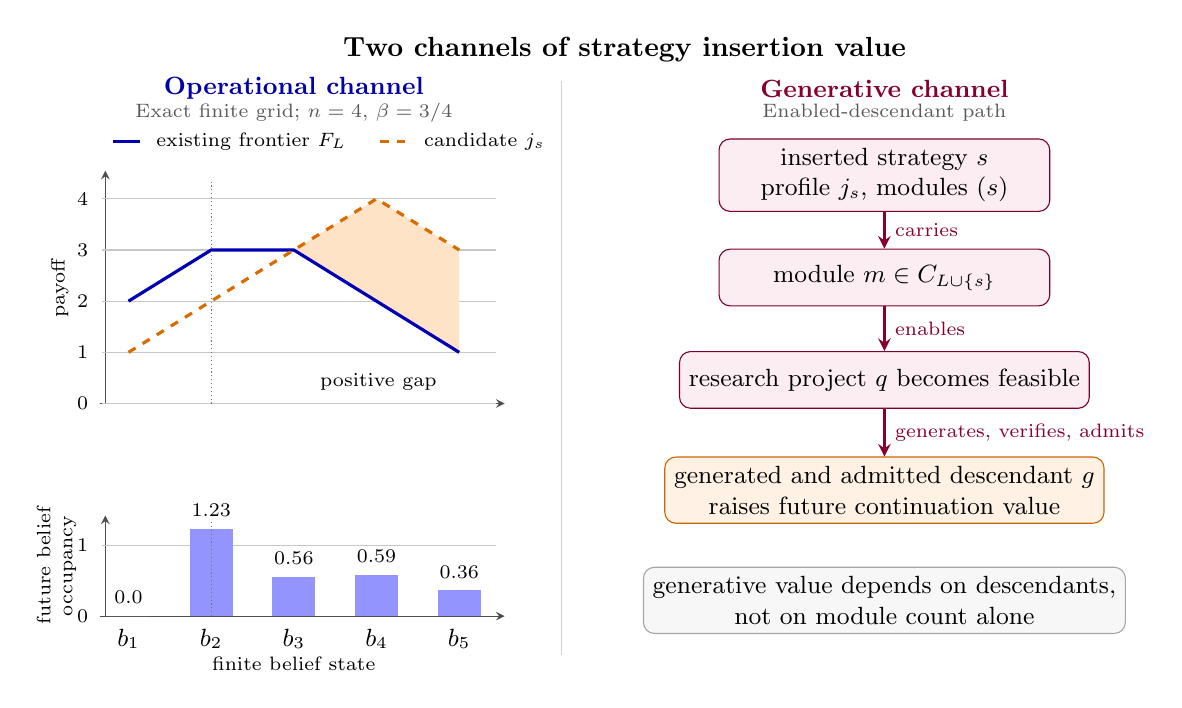
\begin{tikzpicture}[font=\small,>=stealth]
  \node[font=\bfseries] at (7.35,5.85)
    {Two channels of strategy insertion value};

  \node[font=\bfseries\small,text=blue!65!black] at (3.15,5.35)
    {Operational channel};
  \node[font=\scriptsize,text=black!65] at (3.15,5.04)
    {Exact finite grid; \(n=4\), \(\beta=3/4\)};
  \draw[blue!70!black,line width=1.1pt] (0.85,4.68) -- (1.2,4.68);
  \node[font=\scriptsize,anchor=west] at (1.28,4.68)
    {existing frontier \(F_L\)};
  \draw[orange!85!black,line width=1.1pt,dashed] (4.25,4.68) -- (4.6,4.68);
  \node[font=\scriptsize,anchor=west] at (4.68,4.68)
    {candidate \(j_s\)};
  \begin{scope}[xshift=0cm,yshift=1.35cm,x=1.05cm,y=0.65cm]
    \draw[->,black!70] (0.65,0) -- (5.55,0);
    \draw[->,black!70] (0.72,0) -- (0.72,4.55);
    \foreach \y in {0,1,2,3,4} {
      \draw[black!22] (0.68,\y) -- (5.45,\y);
      \node[font=\scriptsize,anchor=east] at (0.63,\y) {\y};
    }
    \fill[orange!22] (3,3.0) -- (4,4.0) -- (5,3.0) -- (5,1.0) -- (4,2.0) -- (3,3.0) -- cycle;
    \draw[blue!70!black,line width=1.15pt] (1,2.0) -- (2,3.0) -- (3,3.0) -- (4,2.0) -- (5,1.0);
    \draw[orange!85!black,line width=1.15pt,dashed] (1,1.0) -- (2,2.0) -- (3,3.0) -- (4,4.0) -- (5,3.0);
    \draw[black!55,densely dotted] (2,0) -- (2,4.35);
    \node[rotate=90,font=\scriptsize] at (0.17,2.25) {payoff};
    \node[font=\scriptsize,anchor=west] at (3.2,0.42) {positive gap};
  \end{scope}

  \begin{scope}[xshift=0cm,yshift=-1.35cm,x=1.05cm,y=0.9cm]
    \draw[->,black!70] (0.65,0) -- (5.55,0);
    \draw[->,black!70] (0.72,0) -- (0.72,1.42);
    \draw[black!22] (0.68,1) -- (5.45,1);
    \node[font=\scriptsize,anchor=east] at (0.63,0) {0};
    \node[font=\scriptsize,anchor=east] at (0.63,1) {1};
    \fill[blue!42] (0.74,0) rectangle (1.26,0.0);
\node[font=\scriptsize,anchor=south] at (1,0.035) {0.0};
\fill[blue!42] (1.74,0) rectangle (2.26,1.229);
\node[font=\scriptsize,anchor=south] at (2,1.264) {1.23};
\fill[blue!42] (2.74,0) rectangle (3.26,0.555);
\node[font=\scriptsize,anchor=south] at (3,0.59) {0.56};
\fill[blue!42] (3.74,0) rectangle (4.26,0.585);
\node[font=\scriptsize,anchor=south] at (4,0.62) {0.59};
\fill[blue!42] (4.74,0) rectangle (5.26,0.365);
\node[font=\scriptsize,anchor=south] at (5,0.4) {0.36};
    \draw[black!55,densely dotted] (2,0) -- (2,1.36);
    \node[font=\small,anchor=north] at (1,-0.04) {$b_{1}$};
\node[font=\small,anchor=north] at (2,-0.04) {$b_{2}$};
\node[font=\small,anchor=north] at (3,-0.04) {$b_{3}$};
\node[font=\small,anchor=north] at (4,-0.04) {$b_{4}$};
\node[font=\small,anchor=north] at (5,-0.04) {$b_{5}$};
    \node[rotate=90,font=\scriptsize,align=center] at (0.13,0.71)
      {future belief\\occupancy};
    \node[font=\scriptsize,anchor=north] at (3,-0.44)
      {finite belief state};
  \end{scope}

  \draw[black!18] (6.55,-1.85) -- (6.55,5.45);
  \node[font=\bfseries\small,text=purple!70!black] at (10.65,5.35)
    {Generative channel};
  \node[font=\scriptsize,text=black!65] at (10.65,5.04)
    {Enabled-descendant path};

  \node[draw=purple!65!black,fill=purple!7,rounded corners,
        align=center,minimum width=4.2cm,minimum height=0.78cm]
        (strategy) at (10.65,4.25)
        {inserted strategy \(s\)\\
         profile \(j_s\), modules \(\mods(s)\)};
  \node[draw=purple!65!black,fill=purple!7,rounded corners,
        align=center,minimum width=4.2cm,minimum height=0.72cm]
        (module) at (10.65,2.95)
        {module \(m\in C_{L\cup\{s\}}\)};
  \node[draw=purple!65!black,fill=purple!7,rounded corners,
        align=center,minimum width=4.2cm,minimum height=0.72cm]
        (project) at (10.65,1.65)
        {research project \(q\) becomes feasible};
  \node[draw=orange!80!black,fill=orange!10,rounded corners,
        align=center,minimum width=4.2cm,minimum height=0.82cm]
        (descendant) at (10.65,0.25)
        {generated and admitted descendant \(g\)\\
         raises future continuation value};

  \draw[->,purple!70!black,line width=1pt] (strategy) -- node[right,font=\scriptsize]
    {carries} (module);
  \draw[->,purple!70!black,line width=1pt] (module) -- node[right,font=\scriptsize]
    {enables} (project);
  \draw[->,purple!70!black,line width=1pt] (project) -- node[right,font=\scriptsize]
    {generates, verifies, admits} (descendant);

  \node[draw=black!35,fill=black!3,rounded corners,align=center,
        minimum width=4.8cm,minimum height=0.75cm]
        at (10.65,-1.15)
        {generative value depends on descendants,\\
         not on module count alone};
\end{tikzpicture}

  \caption{Canonical exact illustration of the estimand
  \(\Delta_n^{\op,\mathrm{aux}}\), the discounted finite-belief gap sum.  The
  candidate has no gap at current belief \(b_2\), but the four-period
  discounted belief occupancy reaches \(b_4\) and \(b_5\), where the
  candidate lies above the existing frontier.  The Julia-generated exact
  rational rows give \(3891/2048\); the five plotted beliefs are discrete and
  joined frontier segments are visual guides only.  The generative arm is a
  model schematic rather than an additional numerical result.}
\end{figure}

The simplest delayed-benefit specialization has two beliefs.  The current
gap is zero, the transition to the second belief is deterministic, and the
second-belief gap is two.  At horizon two with \(\beta=1/2\), the recursion
therefore gives \(0+(1/2)\cdot2=1\).  This example isolates why a strategy can
have zero current payoff advantage yet positive operational value: the
relevant object is discounted belief occupation, not the current belief
alone.
